\documentclass[11pt]{article}
\usepackage[T1]{fontenc}	%special characters
\usepackage[utf8]{inputenc}	%special characters
\usepackage{lmodern,textcomp}% Euro Symbol

\usepackage{hyperref}
\usepackage[margin=1in]{geometry} %article layout margins
\usepackage{tabularx}		%tabulars width fixed textwidth
\usepackage{multicol}	%2 columns in Skills
\usepackage{graphicx}
\usepackage{sectsty}
\sectionfont{
	\sectionrule{0pt}{0pt}{-5pt}{0.8pt}
}

\begin{document}

\Large
\noindent
\textbf{Dirk Hornung, Ph.D.} \\

\normalsize
\noindent
\begin{minipage}{0.5\linewidth}
  \begin{tabularx}{0.6\textwidth}{>{\bfseries}l l}
    City:           & Barcelona \\
    Date of birth:  & October 5, 1991\\
    Place of birth: & Fulda, Germany \\
    Mobile:         & +34 695460404 \\
    E-mail:         & hello@drdirk.io \\
    Website:      	& drdirk.io
  \end{tabularx}
\end{minipage}
\begin{minipage}{0.5\linewidth}
  \begin{flushright}
    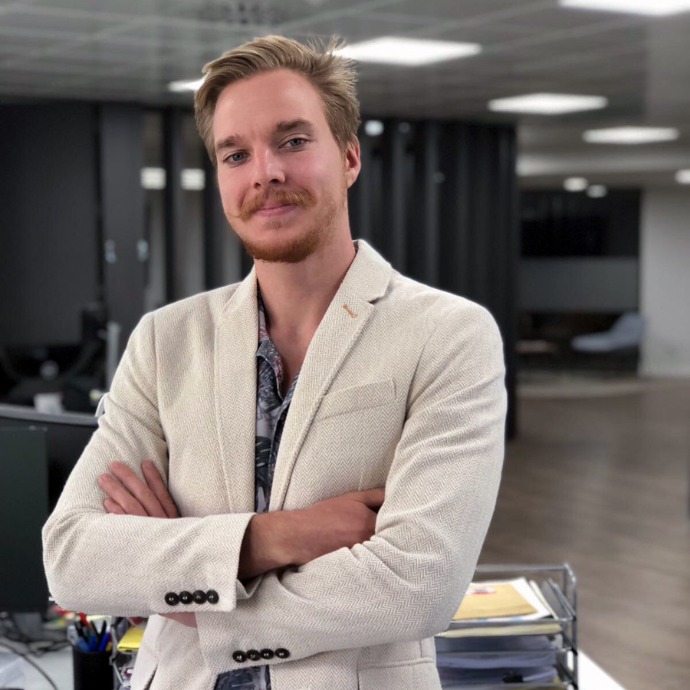
\includegraphics[width=0.4\textwidth]{dirk.png}
  \end{flushright}
\end{minipage}

 \section*{}
 \vspace{1cm}
 Sehr geehrte Frau Rokahr \\

 \noindent Durch meinen ehemaligen Mitbewohner Alexander Kuhn bin auf die
 Tech-Consultancy Senacor gestoßen. Als führender Anbieter für die
 Digitalisierung und individuelle Softwareentwicklung, insbesondere in den
 Bereichen Banking and Insurance, ist Senacor ein attraktiver Arbeitgeber für
 mich, bei dem Ich mich fachlich weiterentwickeln kann. Um meine Karriere auf
 ein neues Level zu heben würde ich gerne als Consultant/ Developer in Ihrem
 Unternehmen einsteigen. \\

\noindent Neben meiner abgeschlossenen Promotion als theoretischer
Teilchenphysiker and der Autonomous University of Barcelona verfüge ich über
vielseitige Praxiserfahrung in der Softwareentwicklung als auch in der
Beratung. So habe ich in den letzten drei Jahren zwei Startups als CTO begleitet
und alle Entscheidungen bezüglich der Software entwicklung selbst getroffen und
umgesetzt. Ersteres Startup war ein Fintech zweiteres ein Legaltech, welches
Softwareberatung und -umsetzung für spanische Anwaltskanzeilen betrieben
hat. Diese Tätigkeiten bestärken mich bei meinem Entschluss als Consultant im
Bereich Banking und Insurance zu arbeiten. \\

\noindent Zu meinen stärken zählt auf der einen Seite das Präsentieren komplexer
Sachverhalte. Um Investitionen zu erhalten oder Kunden zu aquieren müssen
komplexe Ideen eines Startups simple und oft präsentiert werden. Ich habe mit
meinen Präsentationen mehrere Awards gewonnen, wie den besten Fintech Pitch bei
FintechStage, die Aufnahme in diverse Acceleratoren oder den Sieg im Finale des
Adidas Hackathons. Neben dieser stärke bin ich ein erfahrener und
leidenschaftlicher Developer, welcher sich seit seinem 14ten Lebensjahr intensiv
mit der Kunst des Programmierens befasst. Ich habe unzählige Web and Mobile
Applications selbst verwirklicht und beschäfftige mich in den letzen Jahren
ausgiebig mit neuen Technologien wie der Blockchain und der
künstlichen Intelligenz. \\

\noindent Des Weiteren spreche Ich nicht nur fließend Englisch, sondern auch Spanisch und
Französisch, was für Sie von Interesse sein könnte, falls Sie deutschprachige
Digitalisierung in Europa expandieren möchten. \\
 
\noindent Ich freue mich auf eine Einladung zum Vorstellungsgespräch. \\

\noindent Mit freundlichen Grüßen, \\
\noindent Dirk Hornung, PhD

 \end{document}